\documentclass[]{spie}  %>>> use for US letter paper
%\documentclass[a4paper]{spie}  %>>> use this instead for A4 paper
%\documentclass[nocompress]{spie}  %>>> to avoid compression of citations

\renewcommand{\baselinestretch}{1.0} % Change to 1.65 for double spacing
 
\usepackage{amsmath,amsfonts,amssymb}
\usepackage{graphicx}
\usepackage[colorinlistoftodos]{todonotes}
\usepackage{listings}
\lstset{language=Python}
\usepackage[colorlinks=true, allcolors=blue]{hyperref}

\title{Assignment 3:  Solution to Ackley’s Function with Genetic Algorithms and Evolutionary Strategies}

\author{Obed Nehemias Munoz Reynoso (A00354393)
	\\Evolutionary Computing
    \\Master in Computer Science
    \\Monterrey Institute of Technology and Higher Education
}


% Option to view page numbers
\pagestyle{empty} % change to \pagestyle{plain} for page numbers   
\setcounter{page}{301} % Set start page numbering at e.g. 301
 
\begin{document} 
\maketitle

\begin{abstract}
The goal of this assignment is to experiment the (I) implementation of a Genetic Algorithm
(GA) and an Evolutionary Strategy (ES) with adaptive mutation step control, (II) conducting scientific
experiments involving EAs and (III) statistically analyzing experimental results from stochastic algorithms. Both Genetic Algorithm and Evolutionary Strategies will be used for finding an optimal minimal solution for the Ackley Function.
\end{abstract}

% Include a list of keywords after the abstract 
\keywords{Genetic Algorithms, Evolutionary Strategies, Evolutionary Computing}

\section{INTRODUCTION}
\label{sec:intro}  % \label{} allows reference to this section

The Ackley Function is a continuous, multi-modal function obtained by modulating an exponential function
with a cosine wave of moderate amplitude. Originally, it was formulated by Ackley only for the two dimensional case; it is presented here in a generalized, N-dimensional scalable version. Its topology is characterized by an almost flat (due to the dominating exponential) outer region and a central hole or peak where the modulations by the cosine wave become more and more influential. To facilitate its use for minimization and to achieve a standardization of the global minimum to an objective function value of zero, the function is formulated as follows:

$$f(x_0 \cdots x_n) = -20 exp(-0.2 \sqrt{\frac{1}{n} \sum_{i=1}^n x_i^2}) - exp(\frac{1}{n} \sum_{i=1}^n cos(2\pi x_i)) + 20 + e$$ 

$$-32 \leq x_i \leq 32$$ 

$$\text{minimum at }f(0, \cdots, 0) = 0$$

\section{Experiment}
In the above sub-sections, there's a brief description of what are the Genetic Algorithms and Evolutionary Strategies and then some lines of code that represents the most significant parts of their implementation. 

In order to make it a fair play for both Algorithms comparison, mutation is the only way our population will change on every iteration. In this experiment there is not re-combination implementation.

\subsection{Genetic Algorithm}
\label{sec:ga}
Genetic Algorithms are the basics of many of the Evolutionary Solutions for search problems. Genetic Algorithms as a search technique provides a mechanism for finding true or approximate solutions of optimization and search problems. 

\begin{table}[ht]
\caption{ This is a technical summary of main features every Evolutionary technique has and how Genetic Algorithms implement them} 
\label{tab:fonts}
\begin{center}       
\begin{tabular}{|l|l|}
\hline
\rule[-1ex]{0pt}{3.5ex}  Representation & Binary Strings  \\
\hline
\rule[-1ex]{0pt}{3.5ex}  Recombination & N-point or uniform   \\
\hline
\rule[-1ex]{0pt}{3.5ex}  Mutation & Bitwise bit-flipping with fixed probability   \\
\hline
\rule[-1ex]{0pt}{3.5ex}  Parent Selection & Fitness-Proportionate   \\
\hline
\rule[-1ex]{0pt}{3.5ex}  Survivor Selection & All children replace parents   \\
\hline
\rule[-1ex]{0pt}{3.5ex}  Specialty & Emphasis on crossover  \\
\hline
\end{tabular}
\end{center}
\end{table} 

As shown in \textbf{Table 1}, those are the key features for a Simple Genetic Algorithm. In this experiment I did an adjustment in the Representation, it is using real-valued vectors because of the nature of the problem, we need to perform mutations by adding (-1,1) range deltas, it will be easier to perform.
\\
Below is described the main function for Genetic Algorithm with its main functions (initialize, fitness and mutation). 
\\
\begin{lstlisting}[frame=single]  % Start your code-block 
    solution = common.initialize(N,minmax)
    best_fitness = common.fitness(solution[0])

    for gen in range(1, gens):
        if gen % 10 == 0:
            print("Generation :#%d" % gen)

        mutated = mutation.ga_mutation(solution, minmax)
        fitness = common.fitness(mutated[0])

        if fitness <= best_fitness:
            best_fitness = fitness
            solution = mutated
            common.write_data(gen, fitness, 'ga.dat')

        if fitness == 0:
            break
\end{lstlisting}

As we mention before we are not using re-combination. It uses mutation with a simple improvement where we reward the fittest mutated offspring. It means that, if fitness for mutated child is better it will be replacing the old fittest, in other case, it will continue the loop until it finds a fitter child. Below is the mutation function.
\\
\begin{lstlisting}[frame=single]  % Start your code-block 
def ga_mutation(individual, minmax):
    mutated = []
    mutation_idx = random.randint(0, len(individual[0])-1)
    mutation_delta =  round(random.uniform(-1,1),3)
    for idx,value in enumerate(individual[0]):
        if idx == mutation_idx:
            new_value = value + mutation_delta
        else:
            new_value = value
        mutated.append(new_value)
    return (mutated,None)
\end{lstlisting}

\subsection{Evolutionary Strategies}
Evolutionary Strategies are well known for its self-adapted of (mutation parameters) techniques. This fast and a good approach for solving real-valued optimization problems.

\begin{table}[ht]
\caption{ This is a technical summary of main features every Evolutionary technique and how Evolutionary Strategies implement them} 
\label{tab:fonts}
\begin{center}       
\begin{tabular}{|l|l|}
\hline
\rule[-1ex]{0pt}{3.5ex}  Representation & Real-valued vectors \\
\hline
\rule[-1ex]{0pt}{3.5ex}  Recombination & Discrete or Intermediary   \\
\hline
\rule[-1ex]{0pt}{3.5ex}  Mutation & Gaussian Perturbation   \\
\hline
\rule[-1ex]{0pt}{3.5ex}  Parent Selection & Uniform random   \\
\hline
\rule[-1ex]{0pt}{3.5ex}  Survivor Selection & (mu, delta) or (mu + delta)  \\
\hline
\rule[-1ex]{0pt}{3.5ex}  Specialty & Self-adaption of mutation step sized  \\
\hline
\end{tabular}
\end{center}
\end{table} 

From \textbf{Table 2} we took advantage of most of the features it offers. Below the list of implementations:
\begin{itemize}
  \item Real-valued vectors
  \item Mutation using a Gaussian perturbation
  \item Online auto-adjustment of step sizes with the 1/5 Success Rule \cite{auger09}
  \end{itemize}

Below is the main code for execution an Evolutionary Algorithm with the particular feature of applying the 1/5 Success Rule \cite{auger09}
\\
\begin{lstlisting}[frame=single]  % Start your code-block 
    solution = common.initialize(N, minmax)
    best_fitness = common.fitness(solution[0])
    p = 1.5

    for gen in range(1, gens):
        if gen % 10 == 0:
            print("Generation :#%d" % gen)
	        mutated = mutation.es_mutation(solution, minmax, p)
    	fitness = common.fitness(mutated[0])

        if fitness <= best_fitness:
            best_fitness = fitness
            solution = mutated
            p = 1.5
            common.write_data(gen, fitness, 'es.dat')
        else:
            p = 1.5 ** (-1/4)

        if fitness == 0:
            break
\end{lstlisting}
Main ES \textbf{mutation} function
\\
\begin{lstlisting}[frame=single]  % Start your code-block 

def es_mutation(individual, minmax, p):
    new_steps = es_mutate_steps(individual[1], p)
    new_individual = es_mutate_individual(individual, new_steps, minmax)
    return new_individual

\end{lstlisting}

This functions mutates all steps sizes that will be randomly applied in order to generate a new offspring
\begin{lstlisting}[frame=single]  % Start your code-block 
def es_mutate_steps(steps, p):
    steps_size = len(steps)
    new_steps = []
    t1 = np.sqrt(2 * steps_size) ** -1
    t2 = np.sqrt(2 * np.sqrt(steps_size)) ** -1
    for idx,step in enumerate(steps):
        new_step = step * np.exp( (t1 * common.gaussian(0,1))
                                 + (t2 * common.gaussian(0,1)) )

        sigma = new_step * p
        if sigma > 2:
            sigma = sigma % 2
        sigma = 1 - sigma
        new_steps.append(sigma)
    return new_steps
    
\end{lstlisting}

Function where new offspring is generated, it is selecting a random element from the vector and applies the proper step size
\begin{lstlisting}[frame=single]  % Start your code-block 

def es_mutate_individual(individual, steps, minmax):
    data = individual[0]
    new_data = []

    mutated_idx = random.randint(0,len(data))

    for idx,value in enumerate(data):
        if mutated_idx == idx:
            new_value = value + (steps[idx] * common.gaussian(0,1))
        else:
            new_value = value
        new_data.append(common.round(new_value))

    return (new_data, steps)

\end{lstlisting}

\section{Results}
Source code can be obtained from the github repository:
\url{https://github.com/obedmr/ec-ea/tree/master/assigments/assigmt3}

\subsection{Genetic Algorithms}
\begin{verbatim}
$ ./assigmt3.py -n 30 --min -30 --max 30 -g 30000 --strategy ga
.
.
Generation :#29960
Generation :#29970
Generation :#29980
Generation :#29990
#########################
# Strategy              : Genetic Algorithms
# Generations           : 30000
# Best Solution Fitness : 0.010
# Log File              : ./ga.dat
# Graph                 : Genetic_Algorithm_Ackleys_Function.png
#########################
\end{verbatim}
\begin{figure} [ht]
\begin{center}
\begin{tabular}{c} 
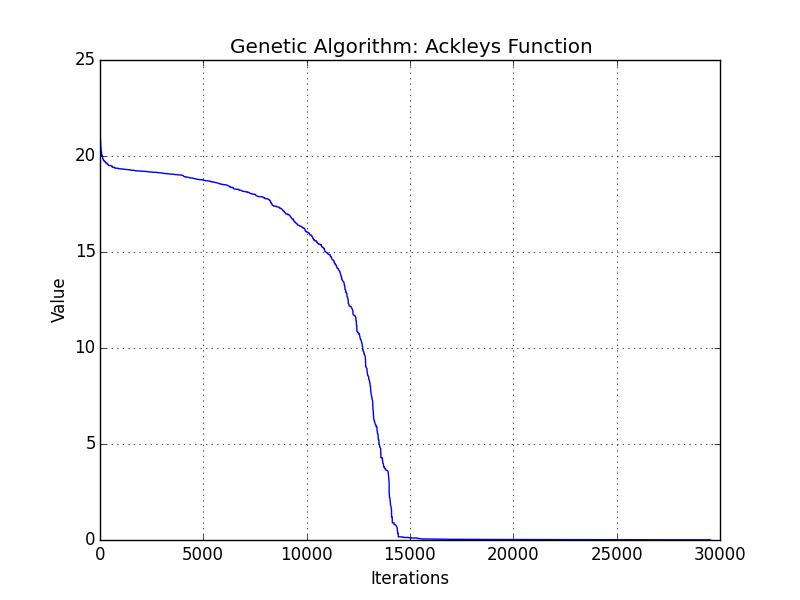
\includegraphics[height=12cm]{Genetic_Algorithm_Ackleys_Function.png}
\end{tabular}
\end{center}
\caption[ga_results] 
{ \label{fig:image-ga} 
Results from Genetic Algorithm execution: \\
\textit{./assigmt3.py -n 30 --min -30 --max 30 -g 30000 --strategy ga}}
\end{figure} 

\subsection{Evolutionary Strategies}

\begin{verbatim}
$ ./assigmt3.py -n 30 --min -30 --max 30 -g 30000 --strategy ga
.
.
Generation :#29960
Generation :#29970
Generation :#29980
Generation :#29990
#########################
# Strategy              : Evolutionary Strategies
# Generations           : 30000
# Best Solution Fitness : 0.007
# Log File              : ./es.dat
# Graph                 : Evolutionary_Strategies_Ackleys_Function.png
#########################

\end{verbatim}

\begin{figure} [ht]
\begin{center}
\begin{tabular}{c} 
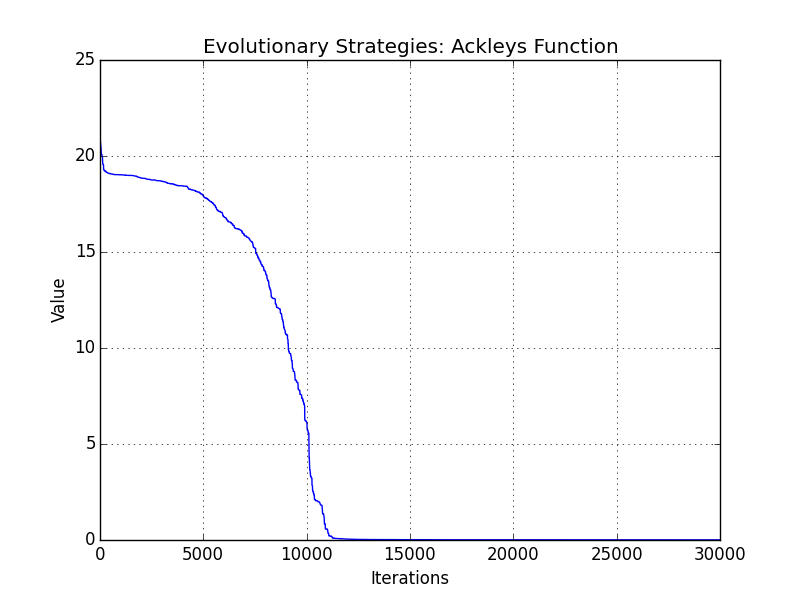
\includegraphics[height=12cm]{Evolutionary_Strategies_Ackleys_Function.png}
\end{tabular}
\end{center}
\caption[es_results] 
{ \label{fig:image-es} 
\textit{Results from Evolutionary Strategies execution: \\
./assigmt3.py -n 30 --min -30 --max 30 -g 30000 --strategy es}}
\end{figure} 

\section{Conclusion}

Even though mutation was the only change method that was implemented, both algorithms performed good in the Ackleys Function minimal search.

Genetic Algorithm: The factor for making it successful was the idea of ignoring to mutate all the offspring that was not fitter at the moment it was mutated.

Evolutionary Strategies: Same as Genetic Algorithm, it implements a single and random selected mutated value from the vector. Also, the application of the 1/5 Success rule \cite{auger09} guided the algorithm to converge faster. The 1/5 Success rule helps in the self-adaption behavior of the Evolutionary Strategies because it considers previous successful fitness before applying the mutation of step sizes.

An extra change was required in our step-size mutation, we performed a module 2 operation in order to obtain a number in the range (0, 2) and then apply a subtract it against 1 in order to obtain (-1, 1) range step sizes. 

\begin{thebibliography}{9}

\bibitem{auger09}
Anne Auger
\emph{\:Benchmarking the (1+1) Evolution Strategy with One-Fifth Success Rule on the BBOB-2009 Function Testbed},
  ACM-GECCO Genetic and Evolutionary Computation,
  Montreal, Canada,
  2009.
  
\bibitem{smith93}
 Eiben, A.E., Smith, James E 
  \emph{\:Introduction to Evolutionary Computing},
  1st edition,
  1993.

\bibitem{stuart09}
Stuart J. Russell, Peter Norvig
\emph{\:Artificial Intelligence: A Modern Approach},
  3rd edition,
  2009.
  
\end{thebibliography}

\end{document} 
